\usepgflibrary{arrows.meta}
\tikzset{
	wave/.pic={
		\foreach \n [evaluate=\n as \neval using .5*\n] in {.5,1,2,3}
			\draw[scale=#1] (-\n,-\neval) arc [start angle=210,end angle=150,radius=\n];
	}
}
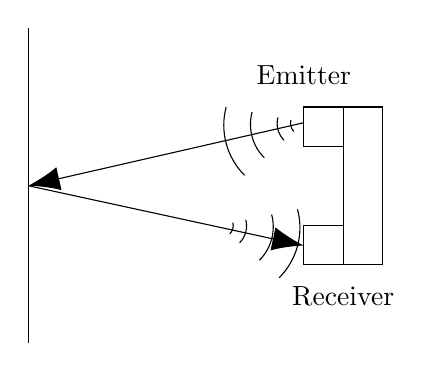
\begin{tikzpicture}[scale=2]
\draw (0,-.5) -- (0,1.5);

\begin{scope}[shift={(2,0)}]
	% labels
	\node at (-.25,1.2) {Emitter};
	\node at (0,-.2) {Receiver};
	% transceiver
	\draw (0,0) rectangle (.25,1);
	\draw (-.25,.75) rectangle (0,1);
	\draw (-.25,0) rectangle (0,.25);
	% sound waves
	\draw (-.25,.9) pic[rotate=15] {wave=.3};
	\draw[x={(-1,0)}] (.8,.12) pic[rotate around={-15:(-1,0)}] {wave=.3};
	% arrows
	\draw[-{Latex[length=4mm]}] (-.25,.9) -- (-2,.5);
	\draw[-{Latex[length=4mm]}] (-2,.5) -- (-.25,.12);
\end{scope}


\end{tikzpicture}
